\documentclass[12pt, a4paper]{report}
\usepackage[utf8]{inputenc}
\usepackage{enumitem}
\usepackage{graphicx}
\graphicspath{ {./images/} }

\usepackage{wasysym}
\usepackage[
backend=biber,
style=alphabetic,
sorting=ynt
]{biblatex}
\addbibresource{tesina.bib}

\usepackage[pdfpagelabels]{hyperref}
\hypersetup{
    plainpages=false,
    colorlinks=true,
    linkcolor=blue,
    filecolor=magenta,
    urlcolor=cyan,
}

\title{Tesina}
\author{Iñaki Garay}
\date{Septiembre 2020}

\begin{document}

\pagenumbering{Alph}
\begin{titlepage}
\maketitle
\thispagestyle{empty}
\end{titlepage}

\pagenumbering{arabic}
\tableofcontents
\thispagestyle{empty}

\newpage

\addcontentsline{toc}{section}{Introducción / Esquema General}
\section*{Introducción / Esquema General}

\begin{itemize}[noitemsep]

\item Los compiladores tradicionales tienen una arquitectura de pipeline.

\item Los editores y entornos de desarrollo modernos usan LSP (Language Server
Protocol). Porque?

\item Una implementacion de LSP require de componentes de compiladores
(especialmente analisis).

\item La arquitectura de pipeline no se adapta bien a estos requerimientos
modernos de reducir tiempos de compilacion y de proveer informacion online
durante edicion.

\item Estos objetivos puede ser logrados mediante compilacion incremental.

\item La compilacion incremental puede ser lograda mediante una arquitectura
basada en queries.

\item La arquitectura basada en queries es implementada tomando inspiracion de
build systems.

\item Rust-analyzer es la segunda implementacion de LSP para rust.

\item Porque no funciono la primera iteracion?

\item Rust-Analyzer usa una libreria, Salsa, para cachear las queries parciales.

\item Como funciona Salsa?

\end{itemize}

\addcontentsline{toc}{section}{Motivaciones}
\section*{Motivaciones}

Los compiladores ya no son cajas negras que ingestan un conjunto de archivos
fuente y producen codigo ensamblador. De compiladores modernos se espera que:

\begin{itemize}[noitemsep]

\item Sean incrementales, es decir, si se recompila el proyecto despues de
producir modificaciones en el código fuente, solo se recompile lo que fue
afectado por esas modificaciones.

\item Provean funcionalidad para editores, e.g. saltar a definición, encontrar
el tipo de una expresión en una ubicación dada, y mostrar errores al editar.

\end{itemize}

\addcontentsline{toc}{subsection}{Arquitecturas Tradicionales de Compiladores}
\subsection*{Arquitecturas Tradicionales de Compiladores}

\noindent
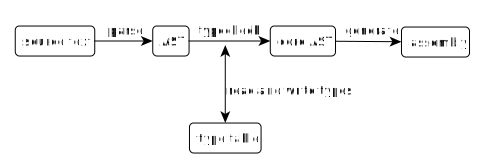
\includegraphics[width=\textwidth]{olle_trad_comp_arq}
\cite{olle_query_based}

Hay muchas variaciones, y frecuentemente mas pasos y representaciones
intermedias que las ilustradas, pero la idea esencial es la misma: se empuja
codigo fuente por un pipeline y corremos un conjunto fijo de transformaciones
hasta que finalmente emitimos codigo ensamblador o algun otro lenguaje. En el
camino frecuentemente se necesita leer y actualizar estado interno. Por ejemplo,
se puede actualizar la tabla de tipos durante la fase de verificacion de tipado,
para que mas adelante se pueda verificar el tipo de las entidades a las cuales
el codigo se refiere. \cite{olle_query_based}

\addcontentsline{toc}{subsection}{Language Server Protocol}
\subsection*{Language Server Protocol}

El Language Server Protocol (LSP) es una protocolo abierto basado en JSON-RPC
para el uso entre editores de codigo fuente o

\begin{verbatim}
The Language Server Protocol (LSP) is an open, JSON-RPC-
based protocol for use between source code editors or
integrated development environments (IDEs) and servers that
provide programming language-specific features. The goal of
the protocol is to allow programming language support to be
implemented and distributed independently of any given
editor or IDE.
\end{verbatim}
\cite{language_server_protocol}

\begin{verbatim}
Adding features like auto complete, go to definition, or
documentation on hover for a programming language takes
significant effort.
Traditionally this work had to be repeated for each
development tool, as each tool provides different APIs for
implementing the same feature.

A Language Server is meant to provide the language-specific
smarts and communicate with development tools over a
protocol that enables inter-process communication.

The idea behind the Language Server Protocol (LSP) is to
standardize the protocol for how such servers and
development tools communicate.
This way, a single Language Server can be re-used in
multiple development tools, which in turn can support
multiple languages with minimal effort.

LSP is a win for both language providers and tooling
vendors!
\end{verbatim}
\cite{language_server_protocol}

\begin{verbatim}
Modern integrated development environments (IDEs) provide
developers with sophisticated features like code completion,
refactoring, navigating to a symbol's definition, syntax
highlighting, and error and warning markers.

For example, in a text-based programming language, a
programmer might want to rename a method read.
The programmer could either manually edit the respective
source code files and change the appropriate occurrences of
the old method name into the new name, or instead use an
IDE's refactoring capabilities to make all the necessary
changes automatically. To be able to support this style of
refactoring, an IDE needs a sophisticated understanding of
the programming language that the program's source is
written in. A programming tool without such an
understanding—for example, one that performs a naive
search-and-replace instead—could introduce errors.
When renaming a read method, for example, the tool should
not replace the partial match in a variable that might be
called readyState, nor should it replace the portion of a
code comment containing the word "already". Neither should
renaming a local variable read, for example, end up
altering similarly named variables in other scopes.

Conventional compilers or interpreters for a specific
programming language are typically unable to provide these
language services, because they are written with the goal of
either transforming the source code into object code or
immediately executing the code. Additionally, language
services must be able to handle source code that is not
well-formed, e.g. because the programmer is in the middle of
editing and has not yet finished typing a statement,
procedure, or other construct. Additionally, small changes
to a source code file which are done during typing usually
change the semantics of the program. In order to provide
instant feedback to the user, the editing tool must be able
to very quickly evaluate the syntactical and semantical
consequences of a specific modification. Compilers and
interpreters therefore provide a poor candidate for
producing the information needed for an editing tool to
consume.

Prior to the design and implementation of the Language
Server Protocol for the development of Visual Studio Code,
most language services were generally tied to a given IDE or
other editor. In the absence of the Language Server
Protocol, language services are typically implemented by
utilizing a tool-specific extension API. Providing the same
language service to another editing tool requires effort to
adapt the existing code so that the service may target the
second editor's extension interfaces.

The Language Server Protocol allows for decoupling language
services from the editor so that the services may be
contained within a general purpose language server. Any
editor can inherit sophisticated support for many different
languages by making use of existing language servers.
Similarly, a programmer involved with the development of a
new programming language can make services for that language
available to existing editing tools. Making use of language
servers via the Language Server Protocol thus also reduces
the burden on vendors of editing tools, because vendors do
not need to develop language services of their own for the
languages the vendor intends to support, as long as the
language servers have already been implemented. The Language
Server Protocol also enables the distribution and
development of servers contributed by an interested
third-party, such as end users, without additional
involvement by either the vendor of the compiler for the
programming language in use or the vendor of the editor to
which the language support is being added.

LSP is not restricted to programming languages. It can be
used for any kind of text-based language, like
specifications or domain-specific languages (DSL).
\end{verbatim}
\cite{language_server_protocol_wiki}

\addcontentsline{toc}{subsection}{Velocidad de Compilación}
\subsection*{Velocidad de Compilación}

\begin{verbatim}
- Improving compile times has actually been a major
development focus after Rust reached 1.0 -- although, up to
this point, much of the work towards this goal has gone into
laying architectural foundations within the compiler and we
are only slowly beginning to see actual results.

- One of the projects that is building on these foundations,
and that should help improve compile times a lot for typical
workflows, is incremental compilation. Incremental
compilation avoids redoing work when you recompile a crate,
which will ultimately lead to a much faster
edit-compile-debug cycle.
\end{verbatim}
\cite{rust_blog_incremental_compilation}

\addcontentsline{toc}{section}{Mecanismos}
\section*{Mecanismos}

\addcontentsline{toc}{subsection}{Compilación Incremental}
\subsection*{Compilación Incremental}

La compilación incremental es una forma de computación incremental aplicada a la
compilación.
En contraste con compiladores comúnes que realizan "builds limpios" y ante un
cambio en el código fuente recompilan todas las unidades de compilación, un
compilador incremental solo recompila las unidades modificadas.
Al construir sobre el trabajo hecho previamente, el compilador incremental evita
la ineficiencia de repetir trabajo ya realizado.
Se puede decir que un compilador incremental reduce la granularidad de las
unidades de compilación tradicionales a la vez que mantiene la semántica del
lenguaje.
\cite{wiki_incremental_compiler}

Muchas herramientas de desarrollo aprovechan compiladores incrementales para
proveer a sus usuarios un entorno mucho mas interactivo.
No es inusual que un compilador incremental sea invocado por cada cambio en un
archivo fuente, de tal manera que el usuario es informado inmediatamente de
cualquier error de compilación causado por sus modificaciones.
Este esquema, en contraste con el modelo de compilación tradicional, acorta el
ciclo de desarrollo considerablemente.
\cite{wiki_incremental_compiler}

Una desventaja de este esquema es que el compilador no puede optimizar
fácilmente el código que compila, dada la localidad y el alcance reducido de los
cambios.
Normalmente esto no es un problema, dado que la optimización del código generado
se aplica solamente al producir un \textit{release build}, instancia en la cual
se puede usar el compilador tradicional.
\cite{wiki_incremental_compiler}

\addcontentsline{toc}{subsection}{Arquitectura Basada en Queries \cite{olle_query_based}}
\subsection*{Arquitectura Basada en Queries \cite{olle_query_based}}

\begin{verbatim}
- Going from pipeline to queries

- What does it take to get the type of a qualified name?

- In a pipeline-based architecture we would just look it up
in the type table.

- With queries, we have to think differently.

- Instead of relying on having updated some piece of state,
we do it as if it was done from scratch.

- As a first iteration, we do it completely from scratch

- We first find out what file the name comes from, which
might be Data/List.vix for Data.List, then read the contents
of the file, parse it, perhaps we do name resolution to find
out what the names in the code refer to given what is
imported, and last we look up the name-resolved definition
and type check it, returning its type.

```
fetchType :: QualifiedName -> IO Type
fetchType (QualifiedName moduleName name) = do
fileName <- moduleFileName moduleName
sourceCode <- readFile fileName
parsedModule <- parseModule sourceCode
resolvedModule <- resolveNames parsedModule
let definition = lookup name resolvedModule
inferDefinitionType definition
```

- Let's first refactor the code into smaller functions:

- Note that each of the functions do everything from scratch
on their own, i.e. they're each doing a (longer and longer)
prefix of the work you'd do in a pipeline.

- I've found this to be a common pattern in my query-based
compilers.

- One way to make this efficient would be to add a
memoisation layer around each function.

- That way, we do some expensive work the first time we
invoke a function with a specific argument, but subsequent
calls are cheap as they can return the cached result.

- This is essentially what we'll do, but we won't use a
separate cache per function, but instead have a central
cache, indexed by the query.
\end{verbatim}
\cite{olle_query_based}

\addcontentsline{toc}{subsection}{Why Incremental Compilation in the First Place? \cite{rust_blog_incremental_compilation}}
\subsection*{Why Incremental Compilation in the First Place? \cite{rust_blog_incremental_compilation}}

\begin{verbatim}
- Much of a programmer's time is spent in an
  edit-compile-debug workflow:
  - you make a small change (often in a single module or
    even function),
  - you let the compiler translate the code into a binary,
    and finally
  - you run the program or a bunch of unit tests in order
    to see results of the change.

- After that it's back to step one, making the next small
change informed by the knowledge gained in the previous
iteration. This essential feedback loop is at the core of
our daily work. We want the time being stalled while waiting
for the compiler to produce an executable program to be as
short as possible.

- Incremental compilation is a way of exploiting the fact
that little changes between compiles during the regular
programming workflow: Many, if not most, of the changes done
in between two compilation sessions only have local impact
on the machine code in the output binary, while the rest of
the program, same as at the source level, will end up
exactly the same, bit for bit.

Incremental compilation aims at retaining as much of those
unchanged parts as possible while redoing only that amount
of work that actually must be redone.
\end{verbatim}
\cite{rust_blog_incremental_compilation}

\addcontentsline{toc}{subsection}{How Do You Make Something "Incremental"? \cite{rust_blog_incremental_compilation}}
\subsection*{How Do You Make Something "Incremental"? \cite{rust_blog_incremental_compilation}}

\begin{verbatim}
- We have already heard that computing something
incrementally means updating only those parts of the
computation's output that need to be adapted in response to
a given change in the computation's inputs.

- One basic strategy we can employ to achieve this is to
view one big computation (like compiling a program) as a
composite of many smaller, interrelated computations that
build up on each other.

- Each of those smaller computations will yield an
intermediate result that can be cached and hopefully re-used
in a later iteration, sparing us the need to re-compute that
particular intermediate result again.
\end{verbatim}
\cite{rust_blog_incremental_compilation}

\addcontentsline{toc}{subsection}{An Incremental Compiler \cite{rust_blog_incremental_compilation}}
\subsection*{An Incremental Compiler \cite{rust_blog_incremental_compilation}}

\begin{verbatim}
- The way we chose to implement incrementality in the Rust
compiler is straightforward: An incremental compilation
session follows exactly the same steps in the same order as
a batch compilation session.

- However, when control flow reaches a point where it is
about to compute some non-trivial intermediate result, it
will try to load that result from the incremental
compilation cache on disk instead.

- If there is a valid entry in the cache, the compiler can
just skip computing that particular piece of data. Let's
take a look at a (simplified) overview of the different
compilation phases and the intermediate results they
produce:

- First the compiler will parse the source code into an
abstract syntax tree (AST). The AST then goes through the
analysis phase which produces type information and the MIR
for each function. After that, if analysis did not find any
errors, the codegen phase will transform the MIR version of
the program into its machine code version, producing one
object file per source-level module. In the last step all
the object files get linked together into the final output
binary which may be a library or an executable.

- So, this seems pretty simple so far: Instead of computing
something a second time, just load the value from the cache.
Things get tricky though when we need to find out if it's
actually valid to use a value from the cache or if we have
to re-compute it because of some changed input.
\end{verbatim}
\cite{rust_blog_incremental_compilation}

\addcontentsline{toc}{subsection}{Seguimiento de Dependencias \cite{olle_query_based}}
\subsection*{Seguimiento de Dependencias \cite{olle_query_based}}

\begin{verbatim}
- Rock, Shake, Salsa

- This functionality is provided by Rock, a library that
packages up some functionality for creating query-based
compilers.

- Rock is an experimental library heavily inspired by Shake
and the Build systems à la carte paper.

- It essentially implements a build system framework, like
- make.

- Build systems have a lot in common with modern compilers
since we want them to be incremental, i.e. to take advantage
of previous build results when building anew with few
changes.

- But there's also a difference: Most build systems don't
care about the types of their queries since they work at the
level of files and file systems.

- Build systems à la carte is closer to what we want.

- There the user writes a bunch of computations, tasks,
choosing a suitable type for keys and a type for values.

- The tasks are formulated assuming they're run in an
environment where there is a function fetch of type Key ->
Task Value, where Task is a type for describing build system
rules, that can be used to fetch the value of a dependency
with a specific key.

- In our above example, the key type might look like this:

- The build system has control over what code runs when we
do a fetch, so by varying that it can do fine-grained
dependency tracking, memoisation, and incremental updates.

- Build systems à la carte is also about exploring what kind
of build systems we get when we vary what Task is allowed to
do, e.g. if it's a Monad or Applicative.

- In Rock, we're not exploring that, so our Task is a thin
layer on top of IO.

- A problem that pops up now, however, is that there's no
satisfactory type for Value.

- We want fetch (ParsedModuleKey "Data.List") to return a
ParsedModule, while fetch (TypeKey "Data.List.map") should
return something of type Type.
\end{verbatim}
\cite{olle_query_based}

\addcontentsline{toc}{subsection}{Indexed queries \cite{olle_query_based}}
\subsection*{Indexed queries \cite{olle_query_based}}

\begin{verbatim}
- Rock allows us to index the key type by the return type of
the query. The Key type in our running example becomes the
following GADT:

data Key a where
  ParsedModuleKey :: ModuleName -> Key ParsedModule
  ResolvedModuleKey :: ModuleName -> Key ResolvedModule
  TypeKey :: QualifiedName -> Key Type

- The fetch function gets the type forall a. Key a -> Task
a, so we get a ParsedModule when we run fetch
(ParsedModuleKey "Data.List"), like we wanted, because the
return type depends on the key we use.

- Now that we know what fetch should look like, it's also
worth revealing what the Task type looks like in Rock, more
concretely.

- As mentioned, it's a thin layer around IO, providing a way
to fetch keys (like Key above):

- The rules of our compiler, i.e. its "Makefile", then
becomes the following function, reusing the functions from
above:

rules :: Key a -> Task a
rules key = case key of
  ParsedModuleKey moduleName ->
    fetchParsedModule moduleName
  ResolvedModuleKey moduleName ->
    fetchResolvedModule moduleName
  TypeKey qualifiedName ->
    fetchType qualifiedName
\end{verbatim}
\cite{olle_query_based}

\addcontentsline{toc}{subsection}{Caching \cite{olle_query_based}}
\subsection*{Caching \cite{olle_query_based}}

\begin{verbatim}
- The most basic way to run a Task in Rock is to directly
call the rules function when a Task fetches a key.

- This results in an inefficient build system that
recomputes every query from scratch.

- But the Rock library lets us layer more functionality onto
our rules function, and one thing that we can add is
memoisation.

- If we do that Rock caches the result of each fetched key
by storing the key-value pairs of already performed fetches
in a dependent hashmap.

- This way, we perform each query at most once during a
single run of the compiler.
\end{verbatim}
\cite{olle_query_based}

\addcontentsline{toc}{subsection}{Verifying dependencies and reusing state \cite{olle_query_based}}
\subsection*{Verifying dependencies and reusing state \cite{olle_query_based}}

\begin{verbatim}
- Another kind of functionality that can be layered onto the
rules function is incremental updates. When it's used, Rock
keeps track of what dependencies a task used when it was
executed (much like Shake) in a table, i.e. what keys it
fetched and what the values were.

- Using this information it's able to determine when it's
safe to reuse the cache from a previous run of the compiler
even though there might be changes in other parts of the
dependency graph.

- This fine-grained dependency tracking also allows reusing
the cache when a dependency of a task changes in a way that
has no effect.

- For example, whitespace changes might trigger a re-parse,
but since the AST is the same, the cache can be reused in
queries that depend on the parse result.
\end{verbatim}
\cite{olle_query_based}

\addcontentsline{toc}{subsection}{Reverse dependency tracking \cite{olle_query_based}}
\subsection*{Reverse dependency tracking \cite{olle_query_based}}

\begin{verbatim}
- Verifying dependencies can be too slow for real-time
tooling like language servers, because large parts of the
dependency graph have to be traversed just to check that
most of it is unchanged even for tiny changes.

- For example, if we make changes to a source file with many
large imports, we need to walk the dependency trees of all
of the imports just to update the editor state for that
single file.

- This is because dependency verification by itself needs to
go all the way to the root queries for all the dependencies
of a given query, which can often be a large proportion of
the whole dependency tree.

- To fix this, Rock can also be made to track reverse
dependencies between queries.

- When e.g. a language server detects that a single file has
changed, the reverse dependency tree is used to invalidate
the cache just for the queries that depend on that file by
walking the reverse dependencies starting from the changed
file.

- Since the imported modules don't depend on that file, they
don't need to be re-checked, resulting in much snappier
tooling!
\end{verbatim}
\cite{olle_query_based}

\addcontentsline{toc}{section}{Caso de Estudio: Rustc}
\section*{Caso de Estudio: Rustc}

Rustc, el compilador de rust, tiene su propia implementacion de queries.

\addcontentsline{toc}{subsection}{Rustc Dependency graphs}
\subsection*{Rustc Dependency graphs}

\begin{verbatim}
- There is a formal method that can be used to model a
computation's intermediate results and their individual
"up-to-dateness" in a straightforward way: dependency
graphs.

- It looks like this: Each input and each intermediate
result is represented as a node in a directed graph. The
edges in the graph, on the other hand, represent which
intermediate result or input can have an influence on some
other intermediate result.

- Note, by the way, that the above graph is a tree just
because the computation it models has the form of a tree. In
general, dependency graphs are directed acyclic graphs

- What makes this data structure really useful is that we
can ask it questions of the form "if X has changed, is Y
still up-to-date?". We just take the node representing Y and
collect all the inputs Y depends on by transitively
following all edges originating from Y. If any of those
inputs has changed, the value we have cached for Y cannot be
relied on anymore.
\end{verbatim}
\cite{rust_blog_incremental_compilation}

\addcontentsline{toc}{subsection}{Dependency Tracking in the Compiler}
\subsection*{Dependency Tracking in the Compiler}

\begin{verbatim}
- When compiling in incremental mode, we always build the
dependency graph of the produced data: every time, some
piece of data is written (like an object file), we record
which other pieces of data we are accessing while doing so.

- The emphasis is on recording here. At any point in time
the compiler keeps track of which piece of data it is
currently working on (it does so in the background in
thread-local memory).

- This is the currently active node of the dependency graph.
Conversely, the data that needs to be read to compute the
value of the active node is also tracked: it usually already
resides in some kind container (e.g. a hash table) that
requires invoking a lookup method to access a specific
entry.

- We make good use of this fact by making these lookup
methods transparently create edges in the dependency graph:
whenever an entry is accessed, we know that it is being read
and we know what it is being read for (the currently active
node).

- This gives us both ends of the dependency edge and we can
simply add it to the graph. At the end of the compilation
sessions we have all our data nicely linked up, mostly
automatically.

- This dependency graph is then stored in the incremental
compilation cache directory along with the cache entries it
describes.

- At the beginning of a subsequent compilation session, we
detect which inputs (=AST nodes) have changed by comparing
them to the previous version. Given the graph and the set of
changed inputs, we can easily find all cache entries that
are not up-to-date anymore and just remove them from the
cache.

- Anything that has survived this cache validation phase can
safely be re-used during the current compilation session.

- There are a few benefits to the automated dependency
tracking approach we are employing. Since it is built into
the compiler's internal APIs, it will stay up-to-date with
changes to the compiler, and it is hard to accidentally
forget about. And if one still forgets using it correctly
(e.g. by not declaring the correct active node in some
place) then the result is an overly conservative, but still
"correct" dependency graph: It will negatively impact the
re-use ratio but it will not lead to incorrectly re-using
some outdated piece of data.

- Another aspect is that the system does not try to predict
or compute what the dependency graph is going to look like,
it just keeps track. A large part of our (yet to be written)
regression tests, on the other hand, will give a description
of what the dependency graph for a given program ought to
look like. This makes sure that the actual graph and the
reference graph are arrived at via different methods,
reducing the risk that both the compiler and the test case
agree on the same, yet wrong, value.
\end{verbatim}
\cite{rust_blog_incremental_compilation}

\begin{verbatim}
- **"Faster! Up to 15% or More."***

- Let's take a look at some of the implications of what
  we've learned so far:
  - The dependency graph reflects the actual dependencies
    between parts of the source code and parts of the output
    binary.
  - If there is some input node that is reachable from many
    intermediate results, e.g. a central data type that is
    used in almost every function, then changing the
    definition of that data type will mean that everything
    has to be compiled from scratch, there's no way around
    it.
- In other words, the effectiveness of incremental
  compilation is very sensitive to the structure of the
  program being compiled and the change being made.
  Changing a single character in the source code might very
  well invalidate the whole incremental compilation cache.
  Usually though, this kind of change is a rare case and
  most of the time only a small portion of the program has
  to be recompiled.
\end{verbatim}
\cite{rust_blog_incremental_compilation}

\addcontentsline{toc}{subsection}{The Current Status of the Implementation}
\subsection*{The Current Status of the Implementation** (09/2019)}

\begin{verbatim}
- For the first spike implementation of incremental
compilation, what we call the alpha version now, we chose to
focus on caching object files.

- Consequently, if this phase can be skipped at least for
part of a code base, this is where the biggest impact on
compile times can be achieved.

- With that in mind, we can also give an upper bound on how
much time this initial version of incremental compilation
can save: If the compiler spends X seconds optimizing when
compiling your crate, then incremental compilation will
reduce compile times at most by those X seconds.

- Another area that has a large influence on the actual
effectiveness of the alpha version is dependency tracking
granularity: It's up to us how fine-grained we make our
dependency graphs, and the current implementation makes it
rather coarse in places. For example, the dependency graph
only knows a single node for all methods in an impl. As a
consequence, the compiler will consider all methods of that
impl as changed if just one of them is changed. This of
course will mean that more code will be re-compiled than is
strictly necessary.
\end{verbatim}
\cite{rust_blog_incremental_compilation}

\addcontentsline{toc}{section}{Caso de Estudio: Rust-analyzer y Salsa}
\section*{Caso de Estudio: Rust-analyzer y Salsa}

Rust-Analyzer utiliza una libreria llamada salsa.

\addcontentsline{toc}{subsection}{Caso de Estudio: Como funciona salsa?}
\subsection*{Caso de Estudio: Como funciona salsa?}

La idea central de salsa es definir el programa como un conjunto de \textit{queries}.
Cada query se usa como una función $K \to V$ que mapea de una clave de tipo $K$ a un valor de tipo $V$.

Las queries en salsa son de dos variedades basicas:
\begin{itemize}[noitemsep]
\item \textbf{Entradas:}
definen los inputs basicos al sistema, los cuales pueden cambiar en cualquier momento.
\item \textbf{Funciones:}
funciones puras (sin efectos secundarios) que transforman las entradas en otros valores.
Los resultados de estas queries se memoizan para evitar recomputarlas.
Cuando se modifican las entradas, salsa determina cuales valores memoizados pueden ser reutilizados y cuales deben ser recomputados.
\end{itemize}

El esquema general de utilizacion de salsa consiste en tres pasos:

\begin{enumerate}[noitemsep]
\item Definir uno o mas grupos de queries que contendran las entradas y las queries requeridas.
Se puede definir mas de un grupo para separar las queries en componentes.
\item Definir las queries.
\item Definir la base de datos, la cual contendra el almacenamiento para las entradas y queries utilizadas.
\end{enumerate}

\addcontentsline{toc}{subsection}{Conclusiones}
\section*{Conclusiones}

\begin{verbatim}
- Most modern languages need to have a strategy for tooling,
and building compilers around query systems seems like an
extremely promising approach to me.

- With queries the compiler writer doesn't have to handle
updates to and invalidation of a bunch of ad-hoc caches,
which can be the result when adding incremental updates to a
traditional compiler pipeline.

- In a query-based system it's all handled centrally once
and for all, which means there's less of a chance it's
wrong.

- Queries are excellent for tooling because they allow us to
ask for the value of any query at any time without worrying
about order or temporal effects, just like a well-written
Makefile.

- The system will compute or retrieve cached values for the
query and its dependencies automatically in an incremental
way.

- Query-based compilers are also surprisingly easy to
parallelise.

- Since we're allowed to make any query at any time, and
they're memoised the first time they're run, we can fire off
queries in parallel without having to think much.

- In Sixty, the default behaviour is for all input modules
to be type checked in parallel.
\end{verbatim}
\cite{olle_query_based}

\begin{verbatim}
- **Future Plans** (09/2019)
- The section on the current status already laid out the two
  major axes along which we will pursue increased efficiency:
  - Cache more intermediate results, like MIR and type
    information, which will allow the compiler to skip more
    and more steps.
  - Make dependency tracking more precise, so that the
    compiler encounters fewer false positives during cache
    invalidation.
\end{verbatim}
\cite{rust_blog_incremental_compilation}

\addcontentsline{toc}{section}{Source Notes}
\section*{Source Notes}

\addcontentsline{toc}{subsection}{Anders Hejlsberg on Modern Compiler Construction}
\subsection*{Anders Hejlsberg on Modern Compiler Construction}

\cite{hejlsberg_modern_compiler_construction}

\addcontentsline{toc}{subsection}{Build Systems a la Carte}
\subsection*{Build Systems a la Carte}

\cite{mokhov2018build}

\addcontentsline{toc}{subsection}{A New Architecture for Building Software}
\subsection*{2016 LLVM Developers’ Meeting: D. Dunbar “A New Architecture for Building Software”}

\cite{dunbar2016}

Overview

compile times impact developers
clang was designed from the beginngin to be a very fast c/c++
that was one of the motivations

the strategy was
- to have a tuned lex and parse implementation
- focused heavily on having a low overhead -O0 path, no unnecesary optimizations on -O0, and do things such as fast instruction selection, etc
- redesigned pch (pre compiled headers), try to pull the minimal amount of data from headers
- integrated the assembler into the compiler, to avoid the time of emitting assembly code and loading it back into the assembler

this proved succesful, clang was 3x faster than gcc
but over time this lead has diminished
in part because gcc itself got faster but mainly because

performance regresses over time because features are added, and tuning can break

improving compile time, options:
- distributed compilation
- improved caching, ideally distributed and shared
- do less work

there are things that in the case of clang could be done today, such as reuse the frontend for compiling several files sharing the same compile flags, allowing the frontend to better chache e.g. file stat calls and other metadata, or build pch for hotly edited files.
while this works, the problem is that there is no control in the compiler over how it is invoked, as this depends on the build system
one proposal is to build a compiler-service, but this presents other problems

How we build software today

for most languages, traditional unix/build system model
- compiler runs as a separate process
- primitive mechanisms for communicating dependencies between biuld systems and the compiler
  - the build system tells us about our inputs andoutpus through command line arguemtns
  - mechanism by which the compiler can write out additional dependencies the build system can ingest, we dont even have a real file format we use for that, we just write out a makefile format and force the build system to ingest it
  - fixed input/output

llbuild - a framework

a new architecture for building software

\addcontentsline{toc}{section}{Fuentes y Referencias}
\section*{Fuentes y Referencias}

\begin{itemize}[noitemsep]

\item General
  \begin{itemize}[noitemsep]
  \item \href{https://www.youtube.com/watch?v=wSdV1M7n4gQ}{\CheckedBox Youtube: Anders Hejlsberg on Modern Compiler Construction} \cite{hejlsberg_modern_compiler_construction}
  \item \href{https://en.wikipedia.org/wiki/Incremental_compiler}{\CheckedBox Wikipedia: Incremental Compiler} \cite{wiki_incremental_compiler}
  \item \href{https://ollef.github.io/blog/posts/query-based-compilers.html}{\CheckedBox Olle Fredriksson: Query-based compiler architectures} \cite{olle_query_based}
  \item \href{https://blog.rust-lang.org/2016/09/08/incremental.html}{\CheckedBox Rust Blog: Incremental Compilation} \cite{rust_blog_incremental_compilation}
  \item \href{https://www.microsoft.com/en-us/research/publication/build-systems-la-carte/}{\Square Build Systems A La Carte} \cite{mokhov2018build}
  \item \href{https://dl.acm.org/doi/10.1145/502949.502889}{\CheckedBox An approach to incremental compilation}
    This is old, from 1984.
  \item \href{https://www.youtube.com/watch?v=b_T-eCToX1I}{\Square Youtube: 2016 LLVM Developers’ Meeting: D. Dunbar “A New Architecture for Building Software”} \cite{dunbar2016}
  \end{itemize}

\item Rustc Dev Guide
  \begin{itemize}[noitemsep]
  \item \href{https://rustc-dev-guide.rust-lang.org/overview.html}{\Square Overview of the Compiler}
  \item \href{https://rustc-dev-guide.rust-lang.org/compiler-src.html}{\Square High-level overview of the compiler source}
  \item \href{https://rustc-dev-guide.rust-lang.org/query.html}{\Square Queries: demand-driven compilation}
    \begin{itemize}[noitemsep]
    \item \href{https://rustc-dev-guide.rust-lang.org/queries/query-evaluation-model-in-detail.html}{\Square The Query Evaluation Model in Detail}
    \item \href{https://rustc-dev-guide.rust-lang.org/queries/incremental-compilation.html}{\Square Incremental compilation}
    \item \href{https://rustc-dev-guide.rust-lang.org/queries/incremental-compilation-in-detail.html}{\Square Incremental Compilation In Detail}
    \item \href{https://rustc-dev-guide.rust-lang.org/incrcomp-debugging.html}{\Square Debugging and Testing Dependencies}
    \item \href{https://rustc-dev-guide.rust-lang.org/queries/profiling.html}{\Square Profiling Queries}
    \item \href{https://rustc-dev-guide.rust-lang.org/salsa.html}{\Square How Salsa works}
    \end{itemize}
  \end{itemize}

\item Rust Analyzer
  \begin{itemize}[noitemsep]
  \item \href{https://rust-analyzer.github.io/}{\Square Rust Analyzer}
  \item \href{https://rust-analyzer.github.io/manual.html}{\Square Manual}
  \item \href{https://rust-analyzer.github.io/blog}{\Square Blog}
  \item \href{https://github.com/rust-analyzer/rust-analyzer/tree/master/docs/dev}{\Square rust-analyzer/tree/master/docs/dev}
  \item \href{https://ferrous-systems.com/blog/rust-analyzer-2019/}{\Square Rust Analyzer in 2018 and 2019}
  \item \href{https://ferrous-systems.com/blog/rust-analyzer-status-opencollective/}{\Square Status of rust-analyzer}
  \item \href{https://blog.logrocket.com/intro-to-rust-analyzer/}{\Square 2020 Intro to Rust Analyzer}
  \item \href{https://dev.to/bnjjj/what-i-learned-contributing-to-rust-analyzer-4c7e}{\Square 2020 What I learned contributing to Rust-Analyzer}
  \item \href{https://www.youtube.com/watch?v=7_7ckOKZCJE}{\Square Youtube: Are we *actually* IDE yet? A look on the Rust IDE Story - Igor Matuszewski}
  \item \href{https://www.youtube.com/watch?v=ANKBNiSWyfc}{\Square Youtube: Rust analyzer guide}
  \item \href{https://www.youtube.com/watch?v=DGAuLWdCCAI}{\Square Youtube: rust analyzer syntax trees}
  \item \href{https://www.youtube.com/watch?v=Lmp3P9WNL8o}{\Square Youtube: rust-analyzer type-checker overview by flodiebold}
  \item \href{https://www.youtube.com/playlist?list=PLXajQV_H-DxLMBt0amcuxgTeOTj6L-YGl}{\Square Youtube: Rust Analyzer Q\&A}
  \end{itemize}

\item Salsa
  \begin{itemize}[noitemsep]
  \item \href{https://salsa-rs.github.io/salsa/}{\Square The Salsa Book}
  \item \href{https://www.youtube.com/playlist?list=PL85XCvVPmGQh0P_VEPVM2ZIlBwl4MQMNY}{\Square Youtube: Incremental Compilation Working Group}
  \item \href{https://www.youtube.com/watch?v=N6b44kMS6OM}{\Square Youtube: Responsive compilers - Nicholas Matsakis - PLISS 2019}
  \item \href{https://www.youtube.com/watch?v=LIYkT3p5gTs}{\Square Youtube: Things I Learned (TIL) - Nicholas Matsakis - PLISS 2019}
  \item \href{https://www.youtube.com/watch?v=_muY4HjSqVw}{\Square Youtube: How Salsa Works (2019.01)}
  \item \href{https://www.youtube.com/watch?v=i_IhACacPRY}{\Square Youtube: Salsa In More Depth (2019.01)}
  \item \href{https://www.youtube.com/watch?v=Xr-rBqLr-G4}{\Square Youtube: RLS 2.0, Salsa, and Name Resolution}
  \end{itemize}

\item Rust Compilation Speed
  \begin{itemize}[noitemsep]
  \item \href{https://vfoley.xyz/rust-compile-speed-tips/}{\Square How to alleviate the pain of Rust compile times}
  \item \href{https://blog.mozilla.org/nnethercote/2016/10/14/how-to-speed-up-the-rust-compiler/}{\Square Nethercote: How to speed up the Rust compiler}
  \item \href{https://blog.mozilla.org/nnethercote/2016/11/23/how-to-speed-up-the-rust-compiler-some-more/}{\Square Nethercote: How to speed up the Rust compiler some more}
  \item \href{https://blog.mozilla.org/nnethercote/2018/04/30/how-to-speed-up-the-rust-compiler-in-2018/}{\Square Nethercote: How to speed up the Rust compiler in 2018}
  \item \href{https://blog.mozilla.org/nnethercote/2018/06/05/how-to-speed-up-the-rust-compiler-some-more-in-2018/}{\Square Nethercote: How to speed up the Rust compiler some more in 2018}
  \item \href{https://blog.mozilla.org/nnethercote/2018/11/06/how-to-speed-up-the-rust-compiler-in-2018-nll-edition/}{\Square Nethercote: How to speed up the Rust compiler in 2018: NLL edition}
  \item \href{https://blog.mozilla.org/nnethercote/2018/05/17/the-rust-compiler-is-getting-faster/}{\Square Nethercote: The Rust compiler is getting faster}
  \item \href{https://blog.mozilla.org/nnethercote/2019/07/25/the-rust-compiler-is-still-getting-faster/}{\Square Nethercote: The Rust compiler is still getting faster}
  \item \href{https://blog.mozilla.org/nnethercote/2019/07/17/how-to-speed-up-the-rust-compiler-in-2019/}{\Square Nethercote: How to speed up the Rust compiler in 2019}
  \item \href{https://blog.mozilla.org/nnethercote/2019/10/11/how-to-speed-up-the-rust-compiler-some-more-in-2019/}{\Square Nethercote: How to speed up the Rust compiler some more in 2019}
  \item \href{https://blog.mozilla.org/nnethercote/2019/12/11/how-to-speed-up-the-rust-compiler-one-last-time-in-2019/}{\Square Nethercote: How to speed up the Rust compiler one last time in 2019}
  \item \href{https://blog.mozilla.org/nnethercote/2020/04/24/how-to-speed-up-the-rust-compiler-in-2020/}{\Square Nethercote: How to speed up the Rust compiler in 2020}
  \item \href{https://blog.mozilla.org/nnethercote/2020/08/05/how-to-speed-up-the-rust-compiler-some-more-in-2020/}{\Square Nethercote: How to speed up the Rust compiler some more in 2020}
  \item \href{https://blog.mozilla.org/nnethercote/2020/09/08/how-to-speed-up-the-rust-compiler-one-last-time/}{\Square Nethercote: How to speed up the Rust compiler one last time}
  \item \href{https://pingcap.com/blog/rust-compilation-model-calamity}{\Square PingCAP Blog: The Rust Compilation Model Calamity}
  \item \href{https://pingcap.com/blog/generics-and-compile-time-in-rust}{\Square PingCAP Blog: Generics and Compile-Time in Rust}
  \item \href{https://pingcap.com/blog/rust-huge-compilation-units}{\Square PingCAP Blog: Rust's Huge Compilation Units}
  \item \href{https://pingcap.com/blog/reasons-rust-compiles-slowly}{\Square PingCAP Blog: A Few More Reasons Rust Compiles Slowly}
  \end{itemize}

\item Miscellaneous
  \begin{itemize}[noitemsep]
  \item \href{https://www.youtube.com/watch?v=S2dK5lLFD_0}{\Square Youtube: Making Fast Incremental Compiler for Huge Codebase - Michał Bartkowiak - code::dive 2019}
  \item \href{https://www.youtube.com/watch?v=JbS8a-Ba0Ck}{\Square Youtube: Starting with Semantics - Sylvan Clebsch - PLISS 2019}
  \item \href{https://www.youtube.com/watch?v=mt6pIpt5Wk0}{\Square Youtube: Polyhedral Compilation as a Design Pattern for Compilers (1/2) - Albert Cohen - PLISS 2019}
  \item \href{https://www.youtube.com/watch?v=3TNT5rFVTUY}{\Square Youtube: Polyhedral Compilation as a Design Pattern for Compilers (2/2) - Albert Cohen - PLISS 2019}
  \item \href{https://www.youtube.com/watch?v=yvlhwZgUPG0}{\Square Youtube: First-Class Continuations: What and Why - Arjun Guha}
  \item \href{https://www.youtube.com/watch?v=n_GhkL8GDAk}{\Square Youtube: Implementing First-Class Continuations by Source to Source Translation - Arjun Guha - PLISS 2019}
  \item \href{https://www.youtube.com/watch?v=Lr4cMmaJHrg}{\Square Youtube: Static Program Analysis (part 1/2) - Anders Møller - PLISS 2019}
  \item \href{https://www.youtube.com/watch?v=6QQSIIvH-F0}{\Square Youtube: Static Program Analysis (part 2/2) - Anders Møller - PLISS 2019}
  \end{itemize}

\end{itemize}

\printbibliography[
heading=bibintoc,
title={Bibliografia}
]

\end{document}
